\chapter{Experimental tests}
\label{chap:ghz-experiments}
This last chapter will be concerned with some of the experimental efforts that have been made to test quantum mechanics against local-realism following the GHZ argument.

We will illustrate the ideal experimental conditions first, then we will report an experiment that has been realized to observe GHZ entanglement and finally we will give reference to a test of quantum mechanics against local-realism.

\section{Ideal experimental conditions}
In this brief section we will present what the ideal experiment to verify quantum mechanics against local-realism would be within the argument presented in Chapter \ref{chap:ghz-theorem}.%rephrasing might be needed. why ideal?

We have noticed in \S \ref{sec:ghz-argument} that the state (\ref{eq:ghz-state}) is an eigenstate of all observables (\ref{eq:xyy-observables}) and (\ref{eq:xxx-observable}), moreover it is easy to prove that all these observables commute with each other. This implies that, in principle, we could verify the quantum mechanical predictions with a single apparatus that measures subsequently the observables (\ref{eq:xyy-observables}) and (\ref{eq:xxx-observable}). In addition, a single run of the experiment would suffice to verify such predictions.

Realizing this experiment would involve putting three particles in state (\ref{eq:ghz-state}) and designing apparatuses that measure the product of three spin components.% (see again Observation \ref{obs:product-vs-single})

To our knowledge no attempt on this approach has been made.

%\begin{observation}
%  SINGLE PRODUCT VS SUBSEQUENT MEASUREMENTS OF PRODUCTS
%\end{observation}

\section{Actual experiments}
In this section we will present an experimental approach that has actually been pursued to verify the quantum mechanical predictions against local-realism.

\subsection{Observation of GHZ entanglement}

\begin{figure}
  \centering
  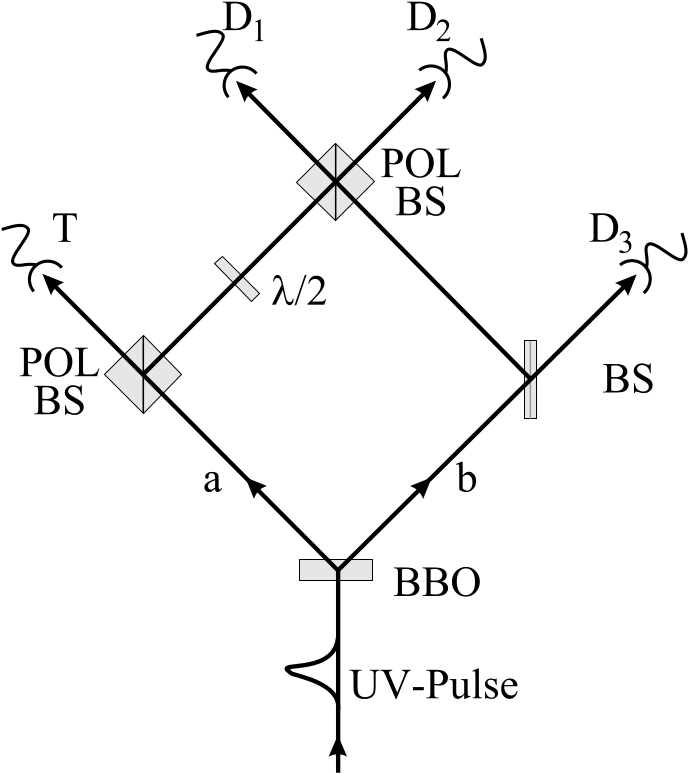
\includegraphics[width=0.4\textwidth]{Mainmatter/Chapter3/ghz-entanglement.png}
  \caption{Experimental set-up for GHZ entanglement demonstration. Credits \cite{PhysRevLett.82.1345}.}
  \label{fig:ghz-entanglement}
\end{figure}

We begin this section by exposing a method that can be used to obtain systems of three particles exhibiting GHZ entanglement \cite{PhysRevLett.82.1345}.

Consider the experimental apparatus schematized in Fig. \ref{fig:ghz-entanglement}. Short pulses of ultraviolet light, which passes through a nonlinear crystal, generate pairs of polarization entangled photons in the state:
\begin{equation}
  \frac{1}{\sqrt{2}} \left( |H\rangle_a |V\rangle_b - |V\rangle_a |H\rangle_b \right),
\end{equation}
where the state $|H\rangle_a |V\rangle_b$ indicates a horizontally polarized photon in arm $a$ and a vertically polarized photon in arm $b$, conversely, the state $|V\rangle_a |H\rangle_b$ indicates a vertically polarized photon in arm $a$ and a horizontally polarized photon in arm $b$.

Continuing along arm $a$ we find a polarizing beam splitter that reflects vertically polarized photons and transmits horizontally polarized photons towards detector $T$. Reflected (vertically polarized) photons go then through a $\lambda/2$ plate that rotates polarization to $45^\circ$, then to a second polarizing beam splitter (analogous to the one already encountered) and finally to detectors $D_1$ ($V$ polarized photons) and $D_2$ ($H$ polarized photons).

Along arm $b$ we find a $50/50$ (polarization independent) beam splitter; transmitted photons go to detector $D_3$ while reflected photons go the second polarizing beam splitter of arm $a$ and finally to detectors $D_1$ ($H$ photons) and $D_2$ ($V$ photons).

All detectors, are behind narrow interference filters, the reason of which will be clarified later.

We want to show here that if two pairs are generated by a single pulse and each of the four photons is detected by one of the detectors $T$, $D_1$, $D_2$ and $D_3$ (exactly one photon per detector) then (with an additional hypothesis we will present in due time) a three photon GHZ state is recorded by detectors $D_1$, $D_2$ and $D_3$. Here is the reasoning: When such a fourfold detection is observed one photon in arm $a$ must have been $H$ polarized. Its companion in arm $b$, $V$ polarized, is either transmitted by the (non polarizing) beam splitter and detected by $D_3$ or reflected and detected by $D_2$ (each possibility with $50 \%$ chance). Consider the former case. Then the other photon in arm $b$, that must be $H$ polarized, is detected by $D_1$ and the last photon, coming through arm $a$, is detected by $D_2$ and is thus $H$ polarized. This situation corresponds to the detection of the state:
\begin{equation}
  |H\rangle_1 |H\rangle_2 |V\rangle_3
  \label{eq:hhv-state}
\end{equation}
by detectors $D_1$, $D_2$ and $D_3$. In the latter case an analogous argument leads us to conclude that the situation corresponds to the detection of the state:
\begin{equation}
  |V\rangle_1 |V\rangle_2 |H\rangle_3.
  \label{eq:vvh-state}
\end{equation}
The two possible states, (\ref{eq:hhv-state}) and (\ref{eq:vvh-state}), that correspond to a fourfold detection will not in general superpose coherently, thus will not give a GHZ state.

The statement we make now is that the lack of coherence is due to the possibility of obtaining information on the pair to which each photon belongs. If we can erase such information then a coherent superposition of the states (\ref{eq:hhv-state}) and (\ref{eq:vvh-state}) will be observed. Let us see why. When a single pulse generates a double pair, these come out from the source in the product state:
\begin{equation}
  \frac{1}{2} \left( |H\rangle_a |V\rangle_b - |V\rangle_a |H\rangle_b \right) \left( |H\rangle'_a |V\rangle'_b - |V\rangle'_a |H\rangle'_b \right).
  \label{eq:double-dc-state}
\end{equation}
The evolution of single components from the source to the detectors $T$, $D_1$, $D_2$ and $D_3$ is given by:
\begin{equation}
  \begin{split}
    |H\rangle_a &\rightarrow |H\rangle_T,\\
    |V\rangle_b &\rightarrow \frac{1}{\sqrt{2}} \left( |V\rangle_2 + |V\rangle_3 \right),\\
    |V\rangle_a &\rightarrow \frac{1}{\sqrt{2}} \left( |V\rangle_1 + |H\rangle_2 \right),\\
    |H\rangle_b &\rightarrow \frac{1}{\sqrt{2}} \left( |H\rangle_1 + |H\rangle_3 \right),
  \end{split}
  \label{eq:single-components-evolution}
\end{equation}
the same holds for the primed states. Substituting these expressions into (\ref{eq:double-dc-state}) and dropping the terms that do not correspond to fourfold detection we obtain, after normalization:
\begin{equation*}
    \frac{1}{2} \left( |H\rangle_T \left( |H\rangle'_1 |H\rangle'_2 |V\rangle_3 + |V\rangle'_1 |V\rangle_2 |H\rangle'_3 \right) + |H\rangle'_T \left( |H\rangle_1 |H\rangle_2 |V\rangle'_3 + |V\rangle_1 |V\rangle'_2 |H\rangle_3 \right) \right)
\end{equation*}
Finally, assuming that primed and unprimed photons are indistinguishable we obtain the state:%is some better comment needed here?
\begin{equation}
  \frac{1}{\sqrt{2}} |H\rangle_T \left( |H\rangle_1 |H\rangle_2 |V\rangle_3 + |V\rangle_1 |V\rangle_2 |H\rangle_3 \right).
  \label{eq:trigger+hv-ghz-state}
\end{equation}

In the experiment considered primed and unprimed photons could, in principle, be distinguished by measuring their energy (the four photon could all have different energies and the sum of the energies of the photons in each pair must be the same for both pairs) and by measuring the delay with which the photons are detected. As an example of this consider the case in which $T$ and $D_3$ fire simultaneously and $D_1$ and $D_2$ also fire simultaneously, this corresponds to one pair being detected by $T$ and $D_3$ and the other pair by $D_1$ and $D_2$. However, if the pulse that generates the two pairs is short and the interference filters behind which the photons are detected have a narrow bandwidth, such possibility of distinction is lost due to the spreading in time of the wave packets. The possibility of distinction by energy measurement is also lost because of the filters.

Experimental demonstration of GHZ entanglement obtained by means of the procedure just presented is reported in the same letter \cite{PhysRevLett.82.1345} which we summarize here.%could be better worded

\begin{figure}
  \centering
  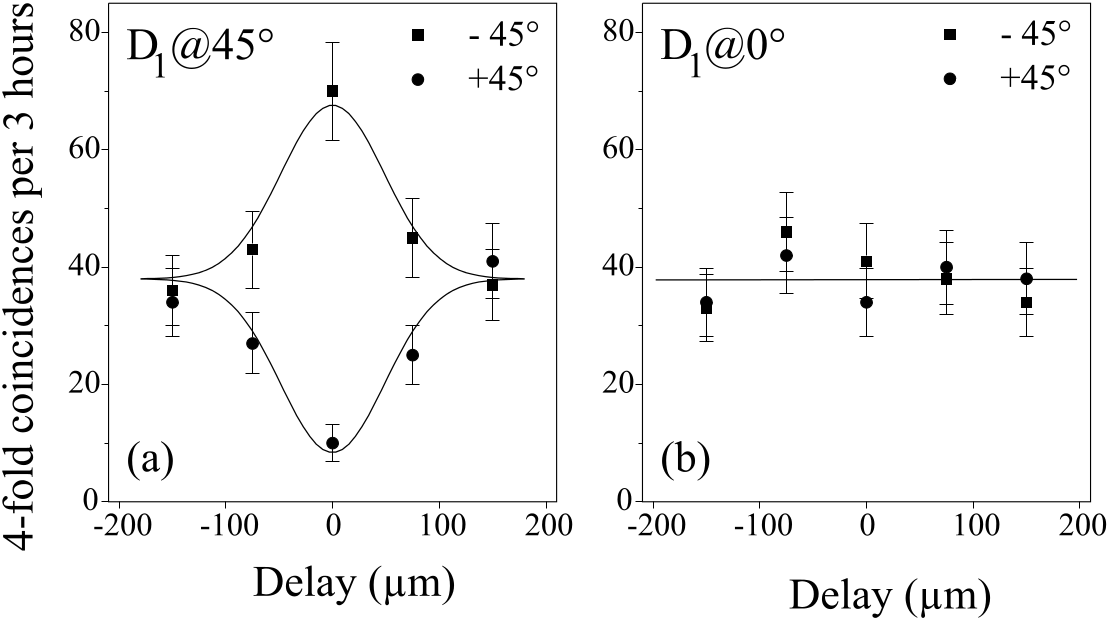
\includegraphics[width=0.6\textwidth]{Mainmatter/Chapter3/ghz-entanglement-exp-proof.png}
  \caption{``Experimental confirmation of GHZ entanglement. Graph (a) shows the results obtained for polarization analysis of the photon at $D_3$, conditioned on the trigger, and the detection of one photon at $D_1$ polarized at $+ 45^\circ$ and one photon at $D_2$ polarized at $- 45^\circ$. The two curves show the fourfold coincidences for a polarizer oriented at $+ 45^\circ$ and $- 45^\circ$, respectively, in front of detector $D_3$ as a function of the spatial delay in path $a$. The difference between the two curves at zero delay confirms the GHZ entanglement. By comparison [graph (b)] no such intensity difference is predicted if the polarizer in front of the detector $D_1$ is set at $0^\circ$.'' Credits \cite{PhysRevLett.82.1345}.}
  \label{fig:ghz-entanglement-exp-proof}
\end{figure}

First of all it is demonstrated that only the two components (\ref{eq:hhv-state}) and (\ref{eq:vvh-state}) are observed. This is done by comparison of the count rates of the eight possible combinations of polarization measurements ($H_1 H_2 H_3$, $H_1 H_2 V_3$, ..., $V_1 V_2 V_3$). A ratio $12:1$ between the expected and unexpected counts is reported. Second, it is demonstrated that the two components (\ref{eq:hhv-state}) and (\ref{eq:vvh-state}) form a coherent superposition (and not a statistical mixture). This is done by measuring the linear polarization of the photon detected by $D_1$ along the $+ 45^\circ$ bisector between the $H$ and $V$ directions. It is easy to show that such a measurement projects the state (\ref{eq:trigger+hv-ghz-state}) into:
\begin{equation*}
  \frac{1}{\sqrt{2}} |H\rangle_T |+ 45^\circ\rangle_1 \left( |H\rangle_2 |V\rangle_3 + |V\rangle_2 |H\rangle_3 \right),
\end{equation*}
that takes the following form when written on the $( |+ 45^\circ\rangle_i, |- 45^\circ\rangle_i), i = 2, 3$ basis:
\begin{equation*}
  \frac{1}{\sqrt{2}} |H\rangle_T |+ 45^\circ\rangle_1 \left( |+ 45^\circ\rangle_2 |+ 45^\circ\rangle_3 - |- 45^\circ\rangle_2 |- 45^\circ\rangle_3 \right).
\end{equation*}
The terms involving $|+ 45^\circ\rangle_2 |- 45^\circ\rangle_3$ and $|- 45^\circ\rangle_2 |+ 45^\circ\rangle_3$ interfere destructively, thus their absence indicates the coherent superposition of terms in (\ref{eq:trigger+hv-ghz-state}).

To show that it is the ``which-path'' information that destroys coherence measures at different delays are taken. This is obtained by varying path $a$ (and thus gradually restoring the possibility of pair distinction).

Fig. \ref{fig:ghz-entanglement-exp-proof} reports experimental results regarding the polarization of photon 3 for fourfold events in which photon 1 and 2 are polarized at $+ 45^\circ$ and $- 45^\circ$ respectively. Squares refer to $- 45^\circ$ polarization and circles to $+ 45^\circ$ polarization.

\begin{observation}
  The argument presented above and the subsequent experimental demonstration show that entanglement doesn't necessarily arise from interaction of the entangled subsystems. We want to give here a general illustration of such a fact taken from \cite{NYAS:NYAS91}.

Consider the factorized two particle state:
\begin{equation}
  |\psi\rangle = |\alpha\rangle_1 |\beta\rangle_2
  \label{eq:factorized-state}
\end{equation}
and the entangled state:
\begin{equation}
  |\Psi\rangle = \frac{1}{\sqrt{2}} \left( |a\rangle_1 |b\rangle_2 + |c\rangle_1 |d\rangle_2\right)
  \label{eq:entangled-state}
\end{equation}
where, for simplicity, $\langle a | c \rangle = \langle b | d \rangle = 0$.
Then, if (\ref{eq:factorized-state}) is not orthogonal to (\ref{eq:entangled-state}), it is possible to obtain an entangled state from (\ref{eq:factorized-state}) using the projection operator:
\begin{equation}
  P = |\Psi\rangle \langle\Psi|.
  \label{eq:projector}
\end{equation}

The experiment presented in this section can be seen as an actual realization of a projector of the type (\ref{eq:projector}). Another example of such a projector that has been experimentally realized is the one used in entanglement swapping experiments which is described in \cite{NYAS:NYAS91}.
\end{observation}

%\begin{observation}
%  ANALOGY WITH DOUBLE SLIT QUANTUM ERASER EXPERIMENT
%\end{observation}


\subsection{Claims regarding local-realism and quantum mechanics}
The experimental observations and analysis we have reported in the previous subsection are not sufficient to make statements against or in favor of local-realism (or quantum mechanics). For example the experimental procedure might be put into question because of the selection needed to isolate fourfold coincidences.

However it has been shown in \cite{PhysRevA.61.022109} that a more refined analysis of the experiment we have presented, together with some additional operational requirements, leads to the possibility of observing violations of local-realism (or of quantum mechanics). In fact claims of having observed such violations (of local-realism) have been made \cite{Nature.403.515}.

The matter of these two last references \cite{PhysRevA.61.022109} and \cite{Nature.403.515} is nevertheless beyond the scope of this thesis and will not be discussed further.

\begin{note}
  It is interesting to note the history of publication of references \cite{PhysRevLett.82.1345}, \cite{PhysRevA.61.022109} and \cite{Nature.403.515}.

  In reference \cite{PhysRevLett.82.1345} no claims regarding local-realism were made. Marek \.{Z}ukowski, informed of the results in \cite{PhysRevLett.82.1345}, carried out a more detailed analysis of the experiment. He found that minor adjustments were to be made in order to be in a position to make such claims \cite{PhysRevA.61.022109}. The same group of \cite{PhysRevLett.82.1345} published \cite{Nature.403.515} less than a month later than \cite{PhysRevA.61.022109}.
\end{note}
